Section~\ref{sec.exp.setup} gives details about our experimental setup for single-fault programs.
In Section~\ref{sec.exp.subject}, we introduce the subject programs used in our study. Sections~\ref{sec.exp.resultsA}~\&~\ref{sec.exp.resultsB} show the results.

\subsubsection{Experimental Setup}\label{sec.exp.setup}

In our experiment, every test case prioritization technique starts from
an arbitrary labeled failed trace because developers start debugging only when
test cases fail.

We compare the effectiveness of different prioritization methods based on the diagnostic cost when the same number of test cases are selected. The diagnostic cost is defined as follows:

\begin{equation}\label{equation.avgcost}
	cost = \dfrac{\left|  \left\{ j \left| \right. f_{T_{\mathcal{S}}}(d_j) \geq f_{T_{\mathcal{S}}}(d_*) \right\}  \right|}{\left|  \mathcal{D} \right|}
\end{equation}

where $\mathcal{D}$ consists of all program elements appearing in the program.
We calculate the average cost as the percentage of elements that developers have
to examine until locating the root cause($d_*$) of failure. Since multiple
program elements can be assigned with the same suspicious score, the numerator
is considered as the number of program elements $d_j$ that have bigger or the
same suspicious score to $d_*$.

In this paper, we use \textsc{Raptor} as the bootstrapping technique ($\mathcal{P}$ in Figure \ref{algo:DMS}). During the bootstrapping process, $w$ is set to 10 to facilitate trend analysis.

Following \cite{JiangCT11}, for each faulty version, we repeat each prioritization technique 20 times to obtain its average cost. For each time, a randomly chosen failed trace is used as the starting point to alleviate the sensitivity of the technique to the choice of starting traces. On the other hand, to fairly compare our approach with other prioritization methods, the {\em same randomly} chosen failed traces are used as the starting traces for all methods.

\subsubsection{Subject Programs}\label{sec.exp.subject}

We use five real {\em C} programs and seven Siemens test programs from the
{\em Software-artifact Infrastructure Repository}~(SIR)~\citep{doESE05}. We refer to the five real programs (\texttt{sed}, \texttt{flex}, \texttt{grep}, \texttt{gzip}, and \texttt{space}) as \textsc{Unix} programs. Table \ref{dataset} shows the descriptive statistics of each subject,
including the number of faults, available test cases and code size. Following many previous studies \citep[e.g.][]{JHS02,Abreu:2009.jss}, we exclude faults not directly observable by the profiling
tool\footnote{http://gcc.gnu.org/onlinedocs/gcc/Gcov.html} (e.g., some faults lead to a crash before \texttt{gcov} dumps profiling information and some faults do not cause any test case to fail), and in total we study 254 faults.

\begin{table}[!htbp]
	%\vspace{-8pt}
	\centering
	\caption{Subject Programs}
	\renewcommand{\arraystretch}{1.5}
	\small
    \begin{tabular}{|l|c|c|c|c|} \hline
        Program & Description & LOC  & Tests & Faults\\ \hline\hline
		tcas & Aircraft Control & 173 & 1609 & 41\\ \hline
        schedule2 & Priority Scheduler & 374  & 2710  & 8\\ \hline
        schedule & Priority Scheduler & 412 & 2651  & 8\\ \hline
        replace & Pattern Matcher & 564 & 5543  & 31\\ \hline
		tot\_info & Info Measure & 565 & 1052  & 22\\ \hline
        print\_tokens2 & Lexical Analyzer & 570  & 4055  & 10\\ \hline
        print\_tokens & Lexical Analyzer & 726 & 4070  & 7\\ \hline
        space & ADL Compiler & 9564 & 1343 & 30\\ \hline
        flex & Lexical Parser & 10124 & 567  & 43\\ \hline
        sed & Text Processor & 9289  & 371  & 22\\ \hline
        grep & Text Processor & 9089 & 809  & 17\\ \hline
        gzip & Data Compressor & 5159 & 217  & 15\\ \hline
	\end{tabular}
	\label{dataset}
\end{table}

\subsubsection{Experimental Results: Reducing Number of Test Cases}\label{sec.exp.resultsA}
%In this subsection, we conduct several controlled experiments to show the effectiveness of \textsc{Dms}.

%\vspace{-4pt}
%\subsubsubsection{Effectiveness on Reducing The Number of Test Cases Needed for a Target Cost}

Here, we investigate the effectiveness of \textsc{Dms} in reducing the number of test cases needed for a target cost. We compare \textsc{Dms} with previous test case prioritization techniques in terms of labeling effort when given an expected fault localization accuracy.
%Since the major objective of our solution is to save labelling effort at the same time retain acceptable fault localization accuracy.
If labeling all test cases and performing fault localization on all program spectra results in an average diagnostic cost $c$, we call it the base line cost. Then we define $x$\% base line effectiveness ($c_x$) as follows:

\begin{equation}\label{equation.accu_cost}
	c_{x} = \frac{x}{100} \times c
\end{equation}

Since Dms would output a ranking list of suspicious code, we compute the  diagnostic cost $c_n$ for Dms when we just inspect top $n$ ($n \in \{1,2,\cdot \cdot \cdot, |D|\}$) suspicious elements. When $c_n$ is less than $c_x$, we record $n$ as the number of labeling effort. Table \ref{tab:label_effort} shows how many labels are needed on average to achieve 101\% base line effectiveness (i.e., within 1\% accuracy lost) for each approach.
E.g., \textsc{Raptor} requires 48 labels on average for each faulty version from the 5 \textsc{Unix} programs while \textsc{Dms} only needs 16.
Overall, \textsc{Dms} requires the minimal amount of labeling effort by achieving 67.7\% labeling reduction on \textsc{Unix}
programs and 10\% reduction on Siemens programs in comparison with the existing best approach (\textsc{Raptor}).

\begin{table}[!htbp]
	%\vspace{-8pt}
	\centering
	\caption{Labeling Effort on Subject Programs}
{
	\scriptsize
		\renewcommand{\arraystretch}{1.5}
%		\hspace{-10pt}
        \begin{tabular}{|m{32pt}|m{13pt}|c|c|m{21pt}|m{21pt}|m{21pt}|m{17pt}|}
		   \hline
		     Subject &             &                &                  & \textsc{Stmt-} & \textsc{Stmt-} & \textsc{Fep-}  & \textsc{Art-} \\
		   Programs & \textsc{Dms} & \textsc{Raptor}  & \textsc{Sequoia} & \textsc{Addtl} & \textsc{Total} & \textsc{Addtl} & \textsc{Min} \\
		   \hline\hline
		   Siemens &   {\bf 18} &         20 &       500\tiny{+} &       500\tiny{+} &       500\tiny{+} &         97 &        150 \\
		   \hline
			\textsc{Unix} &   {\bf 16} &         48 &    176 &        150 &       500\tiny{+} &         98 &         56 \\
		   \hline
		\end{tabular}
}
	\label{tab:label_effort}
\end{table}


%\vspace{-6pt}
\subsubsection{Experimental Results: Reducing Cost}\label{sec.exp.resultsB}
%\subsubsubsection{Effectiveness on Reducing Cost for a Given Number of Labeled Test Cases}

Here, we investigate the effectiveness of \textsc{Dms} in reducing cost given a number of labeled test cases. We select 30 test cases, which we believe are not too many to manually label. We also find that in our experiments the average debugging cost of using \textsc{Dms} will not reduce noticeably even if more labeled test cases are added further (See Figure \ref{Dms_boxplot}). During the bootstrapping process, the first 10 test cases are picked by \textsc{Raptor}. We use different prioritization techniques and apply {\em Ochiai} to evaluate program elements on the selected program spectra. A prioritization technique that obtains a lower cost is better.

\begin{figure}[!htbp]
    \centering
    %\hspace{-0.4cm}
    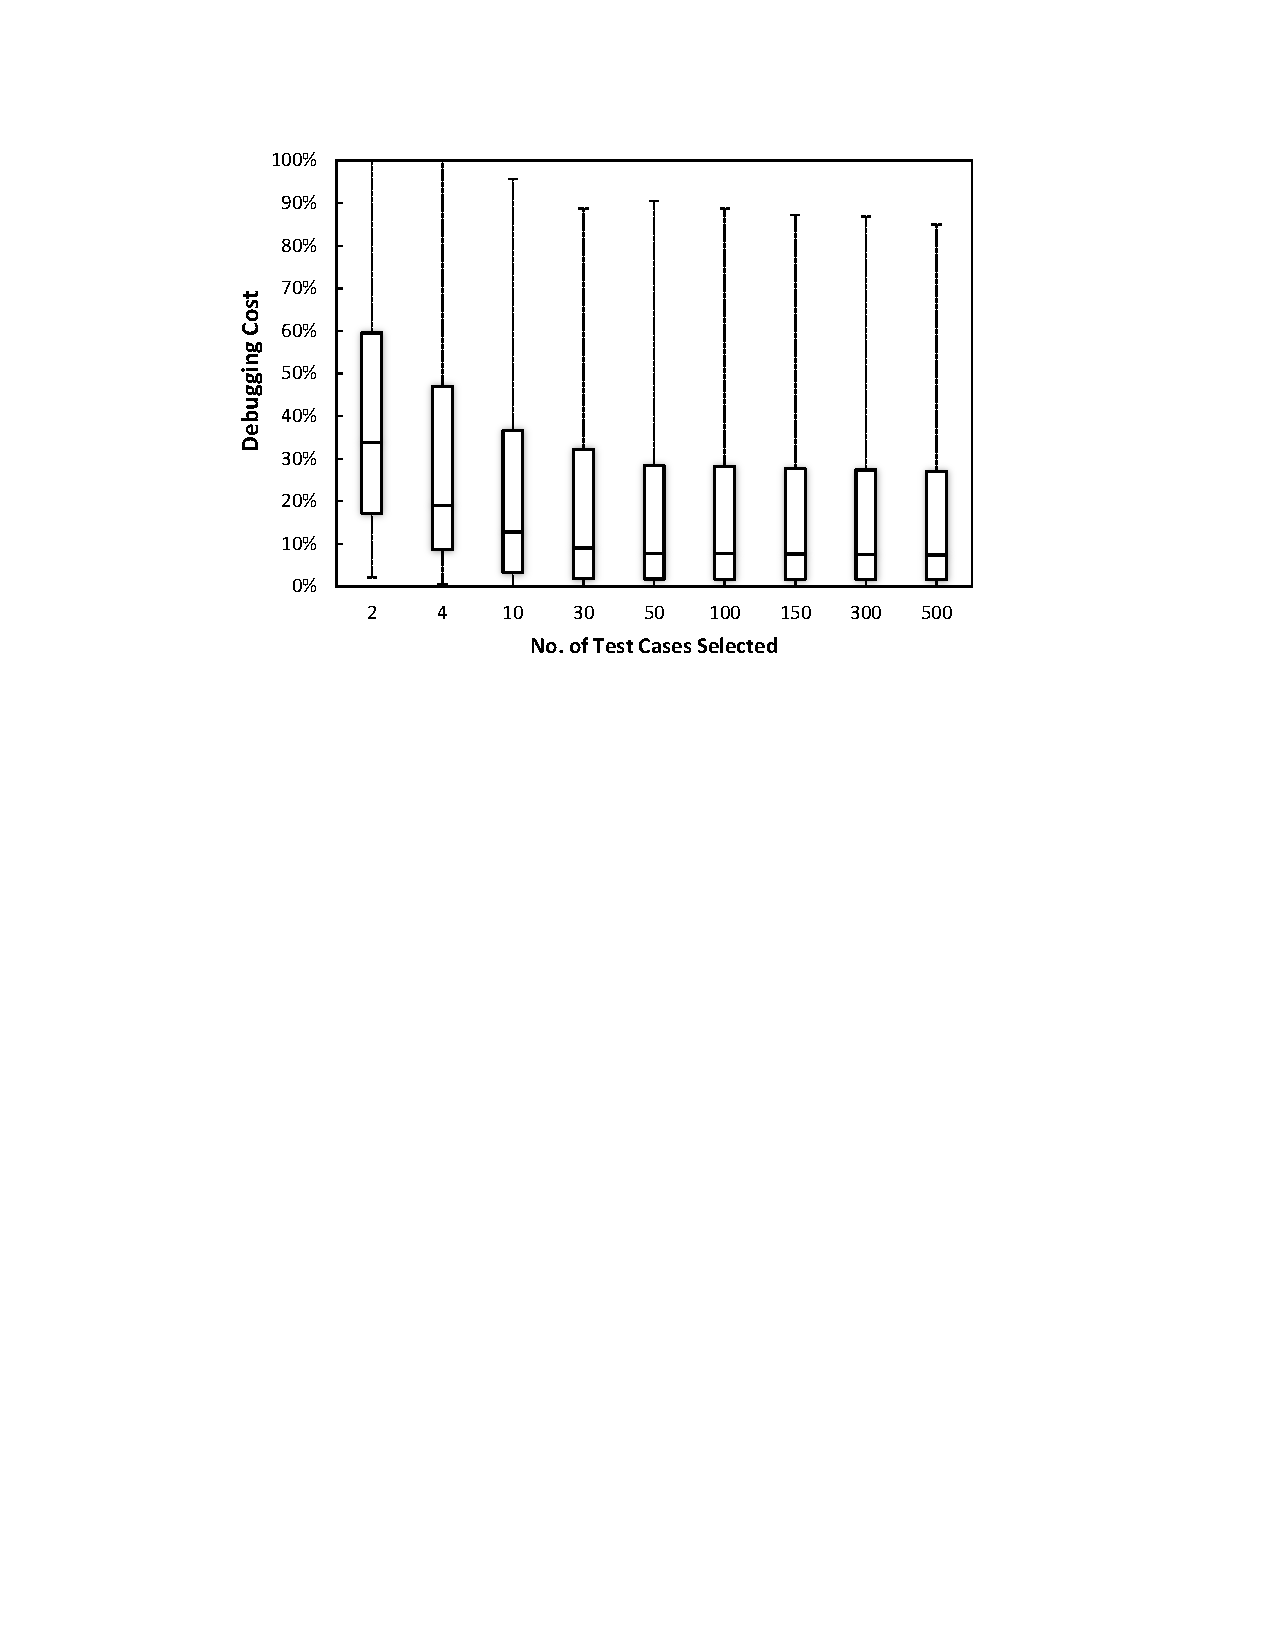
\includegraphics[width=12cm]{sdm_boxplot.pdf}
   % \vspace*{-12pt}
    \caption{Average Cost of {\sc Dms} when Selecting Different Numbers of Test Cases.}
    \label{Dms_boxplot}
\end{figure}

Following \cite{BaahPH10,BaahPH11} and the {\em Cost}
metric (Equation~\ref{equation.avgcost}), we compare
the effectiveness of two prioritization methods $P_A$ and $P_B$ by using
one of the methods (for example, $P_B$) as reference measure.
When selecting equal number of traces $k$, the Cost difference:
$Cost(P_B) - Cost(P_A)$ is considered as the improvement of $P_A$
over $P_B$. A positive value means that $P_A$ performs better than
$P_B$ (since lower Cost is better). The difference corresponds
to the magnitude of improvement. For example, if the Cost of
test cases from $P_A$ is 30\% and the Cost of $P_B$ is 40\%,
then the improvement of $P_A$ over $P_B$ is 10\%, which means
that developers would examine 10\% fewer statements if $P_A$
is deployed.

\vspace{0.2cm}
\noindent{\bf Summary.} Table \ref{tab:compare_11} and \ref{tab:compare_21} summarize the comparison
between our method and the existing prioritizing techniques, the results show that
our method outperforms all of them.

%\vspace{-0.1cm}
\begin{table}[!htbp]
%	\vspace{-8pt}
    \centering
		\caption{Comparison of Prioritization methods.}
		\renewcommand{\arraystretch}{1.5}
		\small
        \begin{tabular}{|c|c|c|c|}
			\hline
			Test Prioritization Method  &  Positive  &  Negative  &   Neutral  \\
			\hline\hline
			\textsc{Dms} vs \textsc{Raptor} & {\bf 25.20\%} &    19.29\% &    55.51\% \\
			\hline
			\textsc{Dms} vs \textsc{Sequoia} & {\bf 33.46\%} &    19.69\% &    46.85\% \\
			\hline
			\textsc{Dms} vs \textsc{Stmt-Addtl} & {\bf 42.13\%} &    19.29\% &    38.58\% \\
			\hline
			\textsc{Dms} vs \textsc{Stmt-Total} & {\bf 62.99\%} &     7.87\% &    29.13\% \\
			\hline
			\textsc{Dms} vs \textsc{Fep-Addtl} & {\bf 40.16\%} &    20.08\% &    39.76\% \\
			\hline
			\textsc{Dms} vs \textsc{Art-Min} & {\bf 31.50\%} &    19.29\% &    49.21\% \\
			\hline
		\end{tabular}
    \label{tab:compare_11}
\end{table}

%\vspace{-0.1cm}
As illustrated in Table \ref{tab:compare_11}, \textsc{Dms} performs
better than \textsc{Raptor} on 25.20\% of the faulty versions, worse
on 19.29\% of the faulty versions, and shows no improvement
on 55.51\% of the faulty versions. The first row of
Table \ref{tab:compare_21} characterizes the degree of positive improvement of
\textsc{Dms} over \textsc{Raptor}. As the table indicates, half of the 33.46\%
faulty versions with positive improvement values have improvements
between 0.03\% and 7.71\%, and the other half
have improvements between 7.71\% and 77.42\%. The average
positive improvement of \textsc{Dms} over \textsc{Raptor} is 7.71\%.

%\vspace{-0.1cm}
\begin{table}[!htbp]
    \centering
		\caption{Distribution of positive improvements.}
		\renewcommand{\arraystretch}{1.5}
		\small
        \begin{tabular}{|c|c|c|c|c|}
			\hline
			Test Pri. Tech.  &        Max &       Mean &     Median &        Min \\
			\hline\hline
			\textsc{Dms} vs \textsc{Raptor} & {\bf 77.42\%} &     7.71\% &     3.93\% &     0.03\% \\
			\hline
			\textsc{Dms} vs \textsc{Sequoia} & {\bf 66.67\%} &    14.38\% &     8.06\% &     0.23\% \\
			\hline
			\textsc{Dms} vs \textsc{Stmt-Addtl} & {\bf 72.87\%} &    14.68\% &     5.17\% &     0.03\% \\
			\hline
			\textsc{Dms} vs \textsc{Stmt-Total} & {\bf 94.97\%} &    27.68\% &    22.29\% &     0.03\% \\
			\hline
			\textsc{Dms} vs \textsc{Fep-Addtl} & {\bf 45.90\%} &    13.83\% &     6.35\% &     0.03\% \\
			\hline
			\textsc{Dms} vs \textsc{Art-Min} & {\bf 53.81\%} &     7.70\% &     3.23\% &     0.03\% \\
			\hline
		\end{tabular}
    \label{tab:compare_21}
\end{table}

We conduct paired Wilcoxon signed-rank test to confirm the difference in performance between \textsc{Dms} and six existing prioritization techniques.
The statistical test result rejects the null hypothesis and suggests that \textsc{Dms} is statistically significantly
better than the existing best approach on \textsc{Unix} programs at 95\% confidence interval.

\vspace{0.2cm}
\noindent{\bf Detailed Comparison.} Table \ref{tab:label_effort} shows that \textsc{Raptor}, \textsc{Fep-Addtl} and \textsc{Art-Min} achieve 101\% base line effectiveness with less than 500 test cases on subject programs.

%Due to limited space, we only show the comparison between \textsc{Dms} and these methods in detail.

Figure~\ref{fig:our_vs_fep}, \ref{fig:our_vs_artmin}, and~\ref{fig:our_vs_ag_unix}
show the comparison between different
prioritization techniques based on fault localization Cost.
The horizontal axes represent the number of versions that
show differences in the Cost of
fault localization. The vertical axes represent the percentage
difference in Costs. If \textsc{Dms} is better than the reference
method, the area above zero-level line will be larger.

\vspace{0.2cm}
\noindent{\bf D{\scriptsize MS} vs F{\scriptsize EP}-A{\scriptsize DDTL}.}
Previous studies~\citep{RUCH01,SEAGMGR01} show that \textsc{Fep-Addtl} is the most
promising prioritizing method for fault detection.
%However \textsc{Fep-Addtl} is not suitable for diagnostic prioritization,
%since it is initially proposed for regression testing, which assumes that
%tester have already get test oracles for each test case. But measuring
%{\em FEP} requires test oracles for all test cases which are absent in our problem.
%As a result, without test oracles {\em FEP} cannot evaluate the fault
%detection rate of each test case on program mutants.
%To circumvent this problem, Alberto \etal~\citep{Gonzalez-SanchezPAGG11} approximated {\em FEP}
Without test oracles, \textsc{Fep} can be estimated by $1 - ${\em False Negative Rate} (\textsc{Fnr})~\citep{Gonzalez-SanchezPAGG11}
\footnote{\textsc{Fnr} is the program passing rate when program element is the real fault and executed in test case. Usually when
\textsc{Fnr} is high, the fault is difficult to be detected by Spectrum-based
fault localization techniques.} which is also used in our study.



\begin{figure}[!htbp]
    \centering
    
\includegraphics[width=12cm]{our_vs_fep.pdf}
%    \vspace{-0.3cm}
    \caption{Improvement of D{\scriptsize MS} over F{\scriptsize EP}-A{\scriptsize DDTL}.}
    \label{fig:our_vs_fep}
\end{figure}
%\vspace{0.2cm}

Figure \ref{fig:our_vs_fep} presents the comparison
between \textsc{Dms} and \textsc{Fep-Addtl} over all faulty versions.
\textsc{Fep-Addtl} is used as the reference prioritization technique.
The baseline represents the fault localization Cost on program spectra prioritized
by \textsc{Fep-Addtl}. Each program version is a bar in this graph and we remove
versions from the graph that have no Cost differences due to the limited space.
In the Figure, the vertical axis represents the magnitude of
improvement of \textsc{Dms} over \textsc{Fep-Addtl}.
If the bar of a faulty version is above the
horizontal axis, that means on this version \textsc{Dms} performs
better than \textsc{Fep-Addtl} (positive improvement) and the bars
below the horizontal axis represent faulty versions for which
\textsc{Dms} performs worse than \textsc{Fep-Addtl}.

The comparison shows that \textsc{Dms} is better than \textsc{Fep-Addtl}.
Out of 153 versions that show differences in Costs, our prioritization method performs
better than \textsc{Fep-Addtl} on 102 versions but performs worse than the
\textsc{Fep-Addtl} on 51 versions.
The positive improvement ranges from 0.03\% to 45.90\%, with an average of 6.35\%.


\begin{figure}[!htbp]
    \centering
    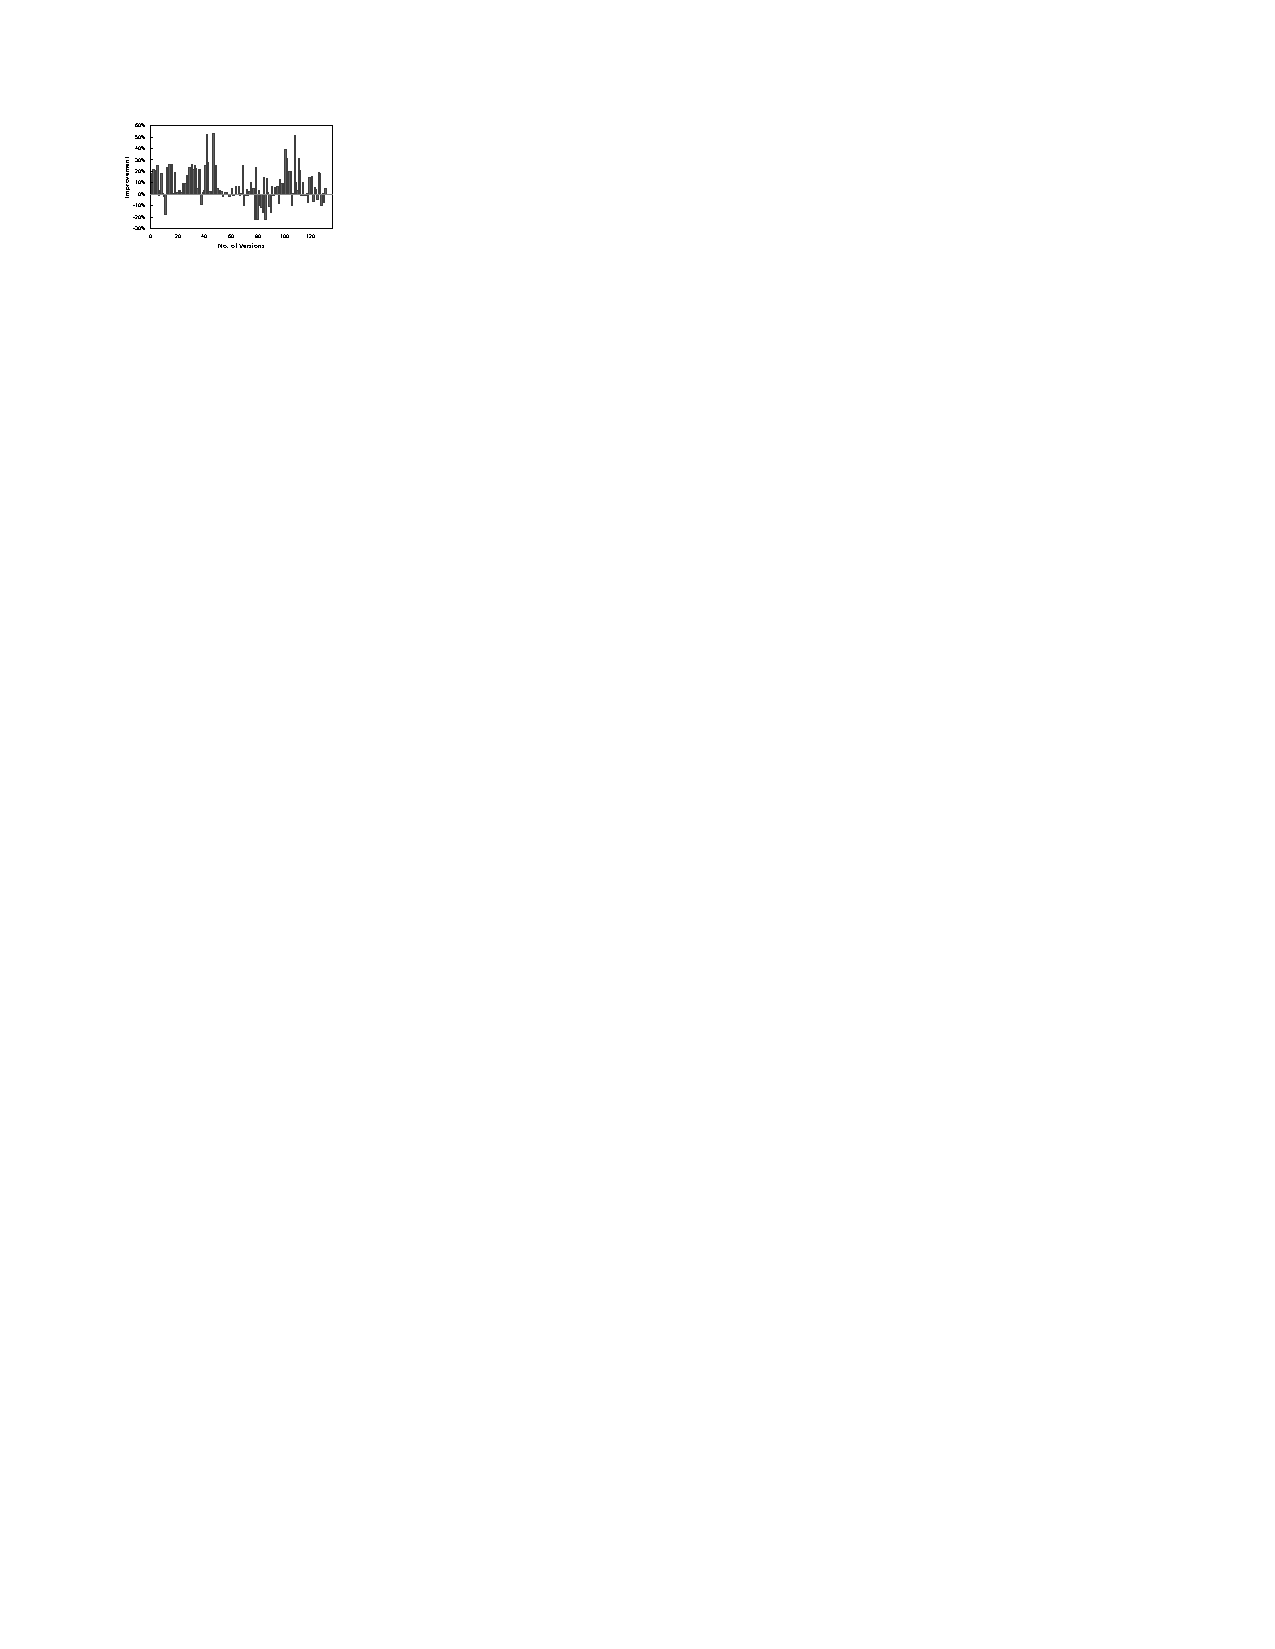
\includegraphics[width=12cm]{our_vs_artmin.pdf}
%    \vspace{-0.3cm}
    \caption{Improvement of D{\scriptsize MS} over A{\scriptsize rt}-M{\scriptsize IN}.}
    \label{fig:our_vs_artmin}
\end{figure}

\vspace{0.2cm}
\noindent{\bf D{\scriptsize MS} vs A{\scriptsize rt}-M{\scriptsize IN}.} In this study we compare the effectiveness of \textsc{Dms} to {\em Adaptive Random Test Prioritization}(\textsc{Art})~\citep{JiangZCT09}.
There are various strategies for \textsc{Art}, in this experiment we only compare with the best one: \textsc{Art-Min}~\citep{JiangZCT09, Gonzalez-SanchezPAGG11, Alberto2011}.
Figure \ref{fig:our_vs_artmin} shows the results of the study in which \textsc{Art-Min} is used
as the baseline method. The comparison shows that \textsc{Dms} is better than \textsc{Art-Min}.
Out of 129 versions that show differences in Costs, our prioritization method performs
better than \textsc{Art-Min} on 80 versions but performs worse than the
\textsc{Art-Min} on 49 versions.
%The positive improvement ranges from 0.03\% to 53.81\%, with an average of 7.70\%.

\vspace{0.2cm}
\noindent{\bf D{\scriptsize MS} vs R{\scriptsize APTOR}.}
Figure \ref{fig:our_vs_ag_unix} shows the comparison between \textsc{Dms} and \textsc{Raptor} on \textsc{Unix} programs.
Here we use \textsc{Raptor} as the reference metric. The comparison shows that \textsc{Dms} is better than \textsc{Raptor}.
On \textsc{Unix} programs \textsc{Dms} outperforms \textsc{Raptor} on 20 versions by at least 1\% cost,
and only 5 versions worse than \textsc{Raptor} over 1\% cost.

\begin{figure}[!htbp]
    \centering
    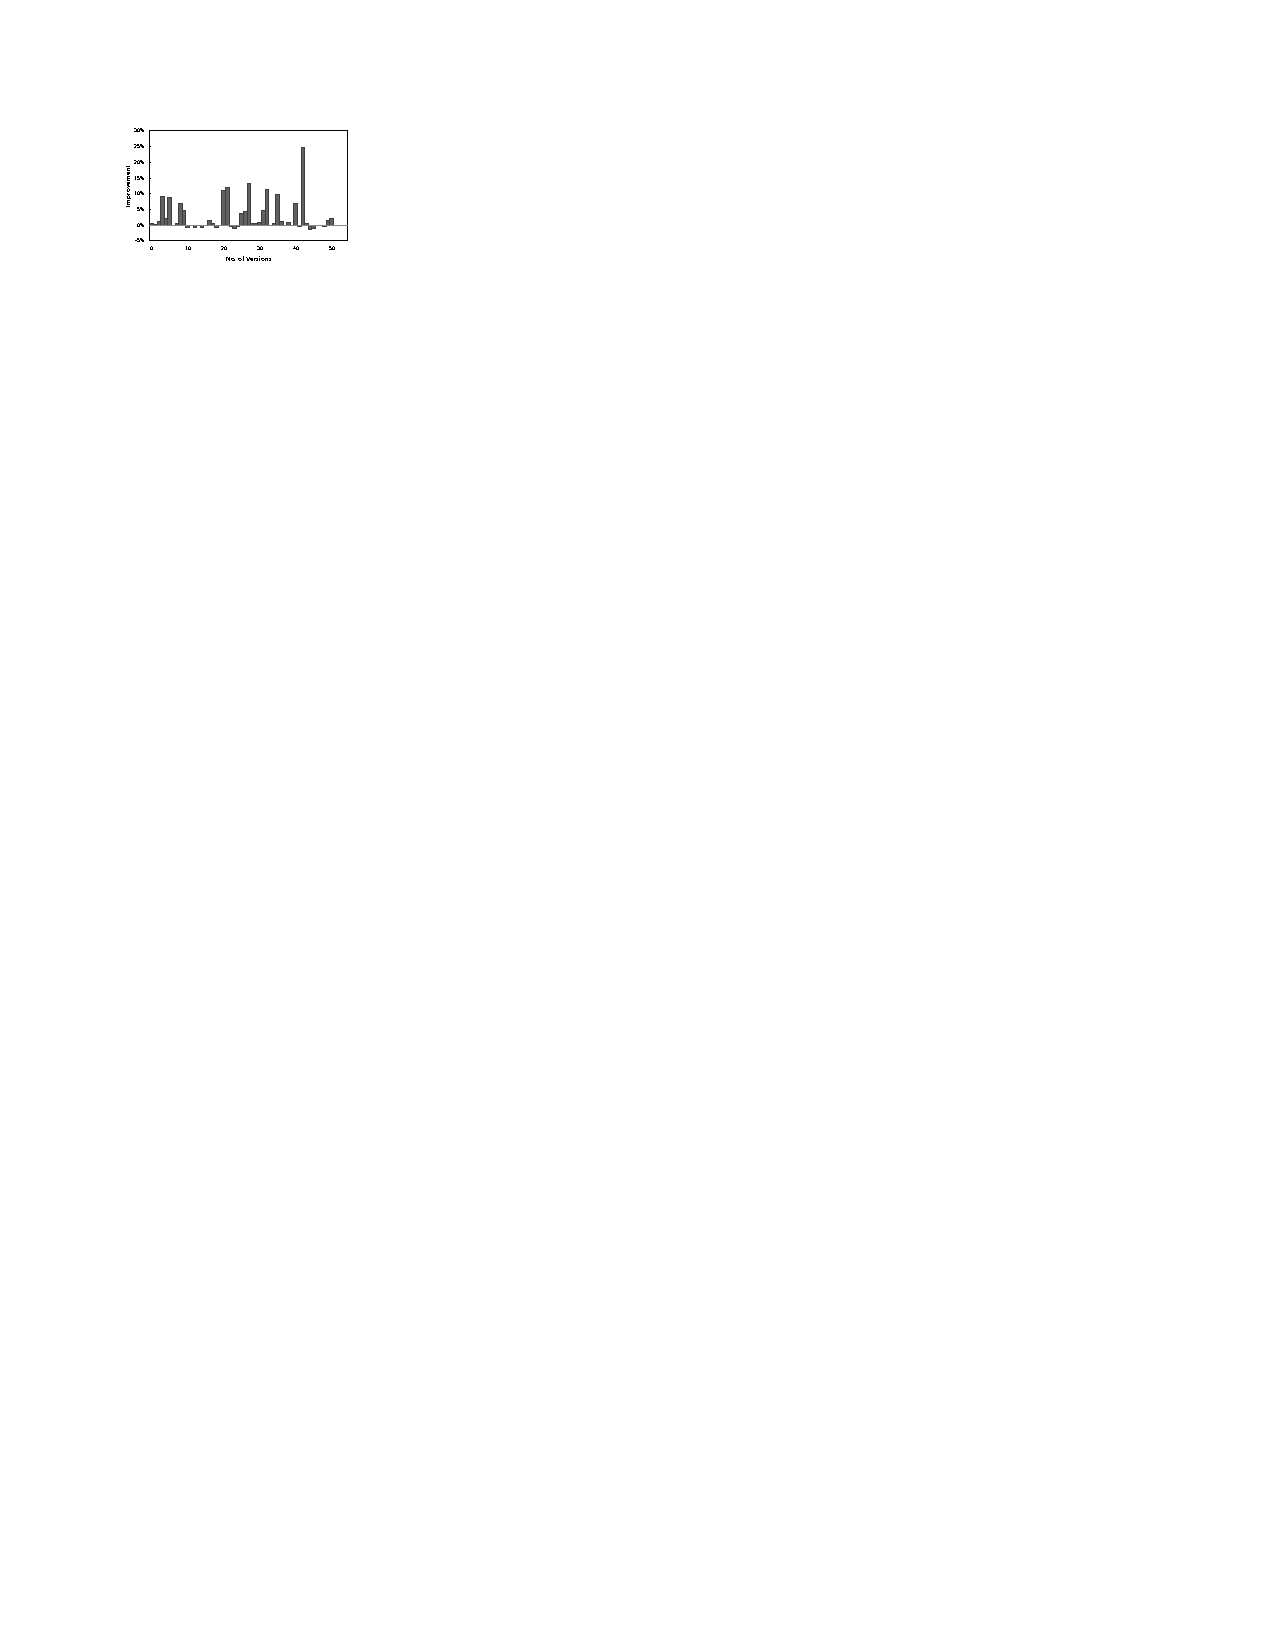
\includegraphics[width=12cm]{our_vs_ag_unix.pdf}
%    \vspace{-0.3cm}
    \caption{Improvement of D{\scriptsize MS} over R{\scriptsize APTOR} on U{\scriptsize NIX} programs.}
    \label{fig:our_vs_ag_unix}
\end{figure}

There is also improvement on Siemens programs: 32.2\% versions show differences and the average debugging cost improvement is 1.3\%, which is not so significant as comparison on \textsc{Unix} programs.
This is probably due to the small software size. On Siemens programs the existing best approach
can reach 101\% of the base line effectiveness by only selecting less than 20 test cases on average (see Table \ref{tab:label_effort}).
By selecting such few test cases, \textsc{Raptor} already obtains the maximal ambiguity group reduction due to very limited different
coverage profiles. For example, all test cases of \texttt{tcas} only have less than 15 ambiguity groups in all faulty versions. In this case,
the speedup by our method is trivial. In real scenario, programs to be diagnosed would be more similar to \textsc{Unix} programs.
